% https://arxiv.org/pdf/1706.03762.pdf
% You only need to write the following sections: 
% 3 Model Architecture
% 5 Training

\documentclass{article}
\usepackage[margin=1.5in]{geometry}
\usepackage{amsmath}
\usepackage{amssymb}
\usepackage{graphicx}
\usepackage{array}

\begin{document}

\section{Model Architecture}
Most competitive neural sequence transduction models have an encoder-decoder structure [5, 2, 35].
Here, the encoder maps an input sequence of symbol representations $(x_1, ..., x_n)$ to a sequence
of continuous representations z = $(z_1, ..., z_n)$. Given z, the decoder then generates an output
sequence $(y_1,\ldots, y_m)$ of symbols one element at a time. At each step the model is auto-regressive
[10], consuming the previously generated symbols as additional input when generating the next.

\setlength{\parskip}{1em}
\noindent
The Transformer follows this overall architecture using stacked self-attention and point-wise, fully
connected layers for both the encoder and decoder, shown in the left and right halves of Figure 1,
respectively

\begin{figure}[htb]
    \centering
    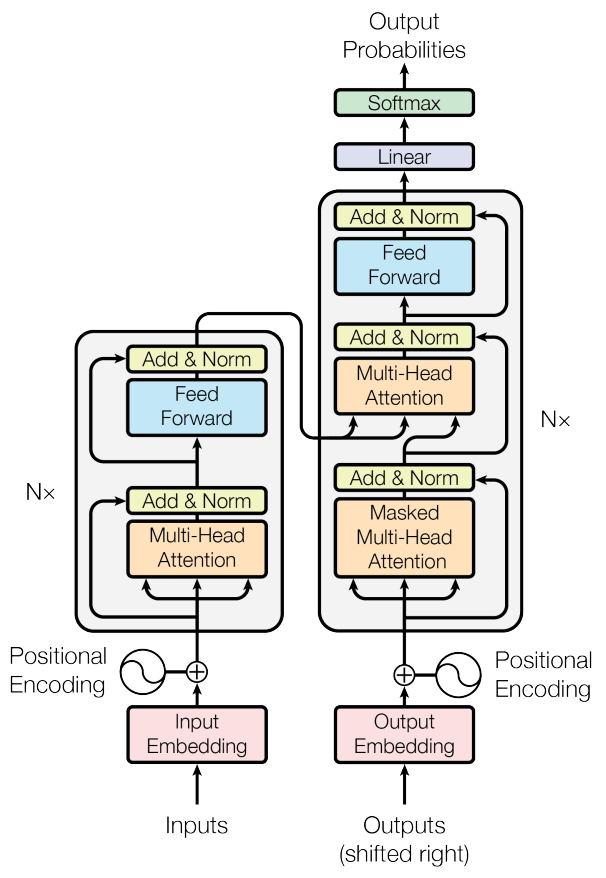
\includegraphics[width=0.5\textwidth]{figures/fig1.PNG}
    \caption{The Transformer - model architecture}
    \label{fig:transformer-architecture}
\end{figure}

\subsection{Encoder and Decoder Stacks}
\textbf{Encoder:} The encoder is composed of a stack of N = 6 identical layers. Each layer has two
sub-layers. The first is a multi-head self-attention mechanism, and the second is a simple, positionwise fully connected feed-forward network. We employ a residual connection [11] around each of
the two sub-layers, followed by layer normalization [1]. That is, the output of each sub-layer is
LayerNorm(x + Sublayer(x)), where Sublayer(x) is the function implemented by the sub-layer
itself. To facilitate these residual connections, all sub-layers in the model, as well as the embedding
layers, produce outputs of dimension dmodel = 512.

\setlength{\parskip}{1em}
\noindent
\textbf{Decoder:} The decoder is also composed of a stack of N = 6 identical layers. In addition to the two
sub-layers in each encoder layer, the decoder inserts a third sub-layer, which performs multi-head
attention over the output of the encoder stack. Similar to the encoder, we employ residual connections
around each of the sub-layers, followed by layer normalization. We also modify the self-attention
sub-layer in the decoder stack to prevent positions from attending to subsequent positions. This
masking, combined with fact that the output embeddings are offset by one position, ensures that the
predictions for position i can depend only on the known outputs at positions less than i.


\subsection{Attention}
An attention function can be described as mapping a query and a set of key-value pairs to an output,
where the query, keys, values, and output are all vectors. The output is computed as a weighted sum
of the values, where the weight assigned to each value is computed by a compatibility function of the
query with the corresponding key.

\begin{figure}[htb]
    \centering
    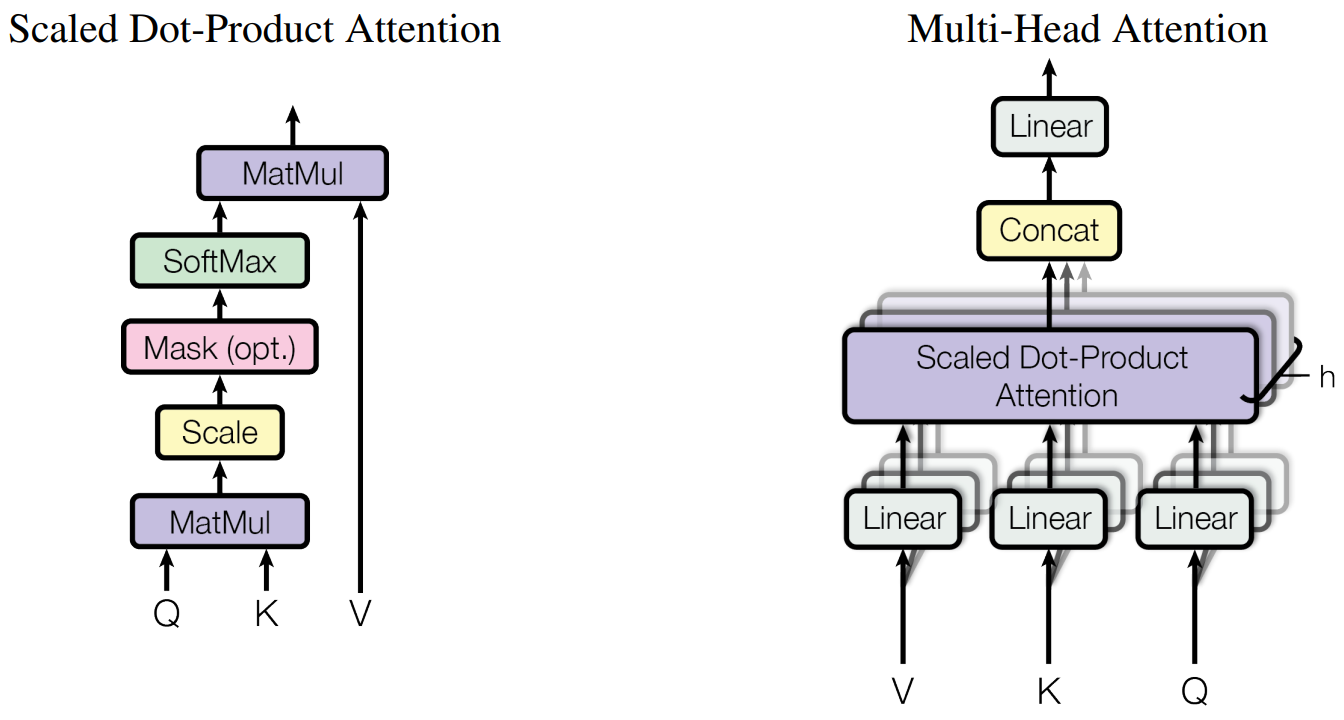
\includegraphics[width=0.5\textwidth]{figures/fig2.PNG}
    \caption{(left) Scaled Dot-Product Attention. (right) Multi-Head Attention consists of several
    attention layers running in parallel.}
    \label{fig:attention}
\end{figure}

\subsubsection{Scaled Dot-Product Attention}
We call our particular attention "Scaled Dot-Product Attention" (Figure 2). The input consists of
queries and keys of dimension dk, and values of dimension dv. We compute the dot products of the
query with all keys, divide each by $\sqrt{d_k}$, and apply a softmax function to obtain the weights on the
values.  

\setlength{\parskip}{1em}
\noindent
In practice, we compute the attention function on a set of queries simultaneously, packed together
into a matrix $Q$. The keys and values are also packed together into matrices $K$ and $V$ . We compute
the matrix of outputs as:
\begin{equation}
    Attention(Q, K, V) = softmax(\frac{QK^\top}{\sqrt{d_k}}) V
\end{equation}
The two most commonly used attention functions are additive attention [2], and dot-product (multiplicative) attention. Dot-product attention is identical to our algorithm, except for the scaling factor
of $\frac{1}{\sqrt{d_k}}$. Additive attention computes the compatibility function using a feed-forward network with
a single hidden layer. While the two are similar in theoretical complexity, dot-product attention is
much faster and more space-efficient in practice, since it can be implemented using highly optimized
matrix multiplication code.

\setlength{\parskip}{1em}
\noindent
While for small values of $d_k$ the two mechanisms perform similarly, additive attention outperforms
dot product attention without scaling for larger values of $d_k$ [3]. We suspect that for large values of
$d_k$, the dot products grow large in magnitude, pushing the softmax function into regions where it has
extremely small gradients\footnote[4]{4To illustrate why the dot products get large, assume 
that the components of q and k are independent random
variables with mean 0 and variance 1. 
Then their dot product $ q \cdot k = \sum_{i = 1}^{d_k} q_i k_i $, has mean 0 and variance $d_k$.}
. To counteract this effect, we scale the dot products by $\frac{1}{\sqrt{d_k}}$

\subsubsection{Multi-Head Attention}
Instead of performing a single attention function with $d_{model}$-dimensional keys, values and queries,
we found it beneficial to linearly project the queries, keys and values $h$ times with different, learned
linear projections to $d_k$, $d_k$ and $d_v$ dimensions, respectively. On each of these projected versions of
queries, keys and values we then perform the attention function in parallel, yielding $d_v$-dimensional
output values. These are concatenated and once again projected, resulting in the final values, as
depicted in Figure~\ref{fig:attention}

\setlength{\parskip}{1em}
\noindent
Multi-head attention allows the model to jointly attend to information from different representation
subspaces at different positions. With a single attention head, averaging inhibits this.
\begin{center}
    Multihead$(Q, K, V)$ = Concat$(head_1, \ldots, head_h)W^O$\\
    where $head_i$ = Attention$(Q_i, K_i, V_i)$
\end{center}
Where the projections are parameter matrices 
$W_i^Q \in \mathbb{R}^{d_{model} \times d_k}$, 
$W_i^K \in \mathbb{R}^{d_{model} \times d_k}$ and 
$W_i^V \in \mathbb{R}^{d_{model} \times d_v}$.

\setlength{\parskip}{1em}
\noindent
In this work we employ $h = 8$ parallel attention layers, or heads. For each of these we use
$d_k = d_v = d_{model}/h = 64$. Due to the reduced dimension of each head, the total computational cost
is similar to that of single-head attention with full dimensionality.

\subsubsection{Applications of Attention in our Model}
The Transformer uses multi-head attention in three different ways:
\begin{itemize}
    \item In "encoder-decoder attention" layers, the queries come from the previous decoder layer,
    and the memory keys and values come from the output of the encoder. This allows every
    position in the decoder to attend over all positions in the input sequence. This mimics the
    typical encoder-decoder attention mechanisms in sequence-to-sequence models such as
    [38, 2, 9].
    \item The encoder contains self-attention layers. In a self-attention layer all of the keys, values
    and queries come from the same place, in this case, the output of the previous layer in the
    encoder. Each position in the encoder can attend to all positions in the previous layer of the
    encoder.
    \item 
\end{itemize}

\subsection{Position-wise Feed-Forward Networks}

\begin{equation}
    FFN(x) = \max(0, xW_1 + b_1)W_2 + b_2
\end{equation}

\subsection{Positional Encoding}

\begin{table}[h]
    \centering
    \caption{Maximum path lengths, per-layer complexity and minimum number of sequential operations
    for different layer types. n is the sequence length, d is the representation dimension, k is the kernel
    size of convolutions and r the size of the neighborhood in restricted self-attention.}
    \label{tab1}
    \begin{tabular*}{\textwidth}{l c >{\centering}p{2cm} c} \\ \hline
        Layer Type & Complexity per Layer 
        & Sequential  Operations 
        & Maximum Path Length \\ \hline
        % row 2
        Self-Attention & $O(n^2 \cdot d)$
        & $O(1)$ & $O(1)$ \\
        % row 3
        Recurrent & $O(n^2 \cdot d)$
        & $O(n)$ & $O(n)$ \\
        % row 4
        Convolutional & $O(k \cdot n \cdot d)$
        & $O(1)$ & $O(log_k(n))$ \\
        % row 5
        Self-Attention(restricted) 
        & $O(r \cdot n \cdot d)$
        & $O(1)$ & $O(n/r)$ \\ \hline
    \end{tabular*}
    
\end{table}

\begin{equation*}
    PE_{(pos, 2i)} = sin(pos/10000^{2i/d_{model}}) \tag {haha}
\end{equation*}
\[
    PE_{(pos, 2i+1)} = cos(pos/10000^{2i/d_{mode}}) \tag{haha1}
\]

\section{Training}
\subsection{Optimier}
\begin{equation}
    lrate = d_{model}^{-0.5} \cdot min(step\_num^{-0.5}, step_num \cdot warmup_steps^{-1.5})
\end{equation}

\subsection{Regularization}
\textbf{Residual Dropout} We apply dropout [33] to the output of each sub-layer, before it is added to the
sub-layer input and normalized. In addition, we apply dropout to the sums of the embeddings and the
positional encodings in both the encoder and decoder stacks. For the base model, we use a rate of
$P_{drop} = 0.1$.
\begin{table}[h]
    \caption{: The Transformer achieves better BLEU scores than previous state-of-the-art models on the
    English-to-German and English-to-French newstest2014 tests at a fraction of the training cost.}

    \begin{tabular*}{\textwidth}{l c c c c} \\ \hline
        Model & \multicolumn{2}{c}{BLEU} & \multicolumn{2}{c}{Training Cost (FLOPs)} \\ 
        \cline{2-3} \space \cline{4-5} 
        & EN-DE & EN-FR &EN-DE & EN-FR  \\ \hline
        ByteNet [18] & 23.75 \\ 
        Deep-Att + PosUnk [39] & & 39.2 & & $1.0 \cdot 10^{20}$ \\
        GNMT + RL [38] & 24.6 & 39.92 & $2.3 \cdot 10^{1}$ & $1.4 \cdot 10^{20}$ \\
        ConvS2S [9] & 25.16 & 40.46 & $9.6 \cdot 10^{18}$ & $1.5 \cdot 10^{20}$ \\
        MoE [32] & 26.03 & 40.56 & $2.0 \cdot 10^{19}$ & $1.2 \cdot 10^{20}$ \\ \hline

        Deep-Att + PosUnk Ensemble [39] & 40.4 & & $8.0 \cdot 10^{20}$ \\
        GNMT + RL Ensemble [38] & 26.30 & 41.16 & $1.8 \cdot 10^{20}$ & $1.1 \cdot 10^{21}$ \\
        ConvS2S Ensemble [9] & 26.36 & \textbf{41.29} & $7.7 \cdot 10^{19}$ & $1.2 \cdot 10^{21}$ \\ 
        \hline
        Transformer (base model) & 27.3 & 38.1 & \multicolumn{2}{c}{\boldmath{$3.3 \cdot 10^{18}$}}  \\
        Transformer (big) & \textbf{28.4} & \textbf{41.8}  & \multicolumn{2}{c}{$2.3 \cdot 10^{19}$} \\
        \hline 
    \end{tabular*}
\end{table}



\end{document}